\begin{refsection} % refsection environment
\chapter[Short title]{Long title}

The table \ref{table:2} is an example of referenced \LaTeX elements.

\begin{table}[h!]
	\centering
	\begin{tabular}{||c c c c||} 
		\hline
		Col1 & Col2 & Col2 & Col3 \\ [0.5ex] 
		\hline\hline
		1 & 6 & 87837 & 787 \\ 
		2 & 7 & 78 & 5415 \\
		3 & 545 & 778 & 7507 \\
		4 & 545 & 18744 & 7560 \\
		5 & 88 & 788 & 6344 \\ [1ex] 
		\hline
	\end{tabular}
	\caption{Table to test captions and labels}
	\label{table:2}
\end{table}


\begin{figure}[ht]
	\centering
	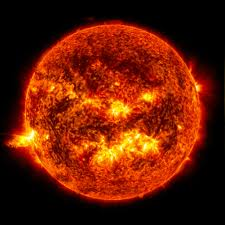
\includegraphics[]{sun.jpg}
	\caption[The sun]{The Sun is the star at the center of the Solar System.}
	\centering
	\label{fig:3}
\end{figure}

The sun(figure \ref{fig:3}), is a ... Also, on page \pageref{fig:3}  we can see...

And in \cite{Piiponniemi2017},...

\addcontentsline{toc}{section}{References}
\printbibliography[heading=subbibliography, title={References}] % print section bibliography
\end{refsection}
